\documentclass[10pt,aspectratio=169,serif]{beamer}

\usepackage[fontset=none, scheme=plain]{ctex}
\IfFontExistsTF{Songti SC}{%
	\setCJKmainfont{Songti SC}[AutoFakeSlant=0.2]%
	\setCJKsansfont{Songti SC}[AutoFakeSlant=0.2]%
}{%
	\setCJKmainfont{FandolSong-Regular}[Extension=.otf,BoldFont=FandolSong-Bold,AutoFakeSlant=0.2]%
	\setCJKsansfont{FandolSong-Regular}[Extension=.otf,BoldFont=FandolSong-Bold]%
}
\usepackage{amsmath,amssymb,graphicx,tikz,booktabs,multicol,calligra}
\usepackage{pgfplots}
\pgfplotsset{compat=1.18}
\usepackage{tcolorbox}
\tcbuselibrary{skins}
\usepackage{XyygU}
\usepackage{caption}
\captionsetup[figure]{name=图,labelsep=period}

\usetikzlibrary{arrows.meta,positioning,calc}

\setlength{\abovedisplayskip}{0pt plus 2pt minus 2pt}
\setlength{\belowdisplayskip}{0pt plus 2pt minus 2pt}

\title[习题3.1]{习题 3.1（复习巩固 \& 综合运用 \& 拓广探索）}
\subtitle{函数的概念与表示法}
\author{}
\institute{}
\date{2026-10-16}

\begin{document}

\begin{frame}
  \titlepage
\end{frame}

% ========== 第1题 ==========
\begin{frame}[t]{第1题：求函数的定义域}
\textbf{1.} 求下列函数的定义域：

\vspace{0.8em}
(1) $\displaystyle f(x)=\frac{3x}{x-4}$；\hfil
(2) $\displaystyle f(x)=\sqrt{x^2}$；

\vspace{1em}
(3) $\displaystyle f(x)=\frac{6}{x^2-3x+2}$；\hfil
(4) $\displaystyle f(x)=\frac{\sqrt{4-x}}{x-1}$。
\end{frame}

\begin{frame}[t]{第1题 解答}
\begin{tcolorbox}[colback=orange!10,colframe=orange,title=\textbf{解}]
(1) 分母 $x-4\neq 0$，即 $x\neq 4$。定义域：$\mathbf{R}\setminus\{4\}$。

\vspace{1em}
(2) $x^2\ge 0$ 对任意实数 $x$ 都成立。定义域：$\mathbf{R}$。

\vspace{1em}
(3) $x^2-3x+2=(x-1)(x-2)\neq 0$，即 $x\neq 1$ 且 $x\neq 2$。定义域：$(-\infty,1)\cup(1,2)\cup(2,+\infty)$。

\vspace{1em}
(4) 需 $\begin{cases}4-x\ge 0,\\ x-1\neq 0,\end{cases}$ 即 $\begin{cases}x\le 4,\\ x\neq 1.\end{cases}$
定义域：$(-\infty,1)\cup(1,4]$。
\end{tcolorbox}
\end{frame}

% ========== 第2题 ==========
\begin{frame}[t]{第2题：同一函数的判断}
\textbf{2.} 下列哪一组中的函数 $f(x)$ 与 $g(x)$ 是同一个函数？

\vspace{0.8em}
(1) $f(x)=x-1$，$\displaystyle g(x)=\frac{x^2}{x}-1$；

\vspace{0.8em}
(2) $f(x)=x^2$，$g(x)=(\sqrt{x})^4$；

\vspace{0.8em}
(3) $f(x)=x^2$，$\displaystyle g(x)=\sqrt[3]{x^6}$。
\end{frame}

\begin{frame}[t]{第2题 解答}
\begin{tcolorbox}[colback=orange!10,colframe=orange,title=\textbf{解}]
(1) $f(x)=x-1$ 的定义域为 $\mathbf{R}$；$g(x)=\dfrac{x^2}{x}-1=x-1$ 要求 $x\neq 0$，定义域为 $\mathbf{R}\setminus\{0\}$。\alert{不是}同一函数。

\vspace{1em}
(2) $f(x)=x^2$ 的定义域为 $\mathbf{R}$；$g(x)=(\sqrt{x})^4=x^2$ 要求 $x\ge 0$，定义域为 $[0,+\infty)$。\alert{不是}同一函数。

\vspace{1em}
(3) $g(x)=\sqrt[3]{x^6}=x^2$，定义域为 $\mathbf{R}$，与 $f(x)=x^2$ 的定义域和对应关系都相同。\alert{是}同一函数。
\end{tcolorbox}
\end{frame}

% ========== 第3题 ==========
\begin{frame}[t]{第3题：画图象并求定义域、值域}
\textbf{3.} 画出下列函数的图象，并说出函数的定义域、值域：

\vspace{0.8em}
(1) $y=3x$；\hfil (2) $\displaystyle y=\frac{8}{x}$；

\vspace{0.8em}
(3) $y=-4x+5$；\hfil (4) $y=x^2-6x+7$。
\end{frame}

\begin{frame}[t]{第3题 解答}
\begin{tcolorbox}[colback=orange!10,colframe=orange,title=\textbf{解}]
(1) $y=3x$：过原点的直线。定义域 $\mathbf{R}$，值域 $\mathbf{R}$。

\vspace{1em}
(2) $y=\dfrac{8}{x}$：双曲线。定义域 $(-\infty,0)\cup(0,+\infty)$，值域 $(-\infty,0)\cup(0,+\infty)$。

\vspace{1em}
(3) $y=-4x+5$：斜率为 $-4$ 的直线。定义域 $\mathbf{R}$，值域 $\mathbf{R}$。

\vspace{1em}
(4) $y=x^2-6x+7=(x-3)^2-2$：开口向上的抛物线，顶点 $(3,-2)$。定义域 $\mathbf{R}$，值域 $[-2,+\infty)$。
\end{tcolorbox}
\end{frame}

\begin{frame}[t]{第3题 图象}
	\vspace{-1em}
\begin{center}
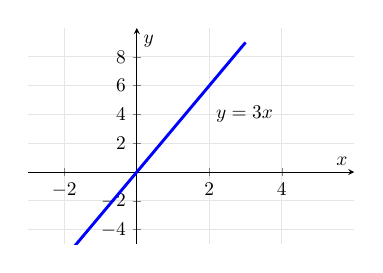
\begin{tikzpicture}[scale=0.7]
\begin{axis}[
    width=7.5cm, height=5.5cm,
    axis lines=middle,
    xlabel=$x$, ylabel=$y$,
    xmin=-3, xmax=6, ymin=-5, ymax=10,
    xtick={-2,0,2,4}, ytick={-4,-2,2,4,6,8},
    grid=major, grid style={gray!20},
]
\addplot[line width=1.5pt,blue,domain=-2:3,samples=2] {3*x};
\node[anchor=west] at (2,4){$y=3x$};

\end{axis}
\end{tikzpicture}
\hspace{2cm}
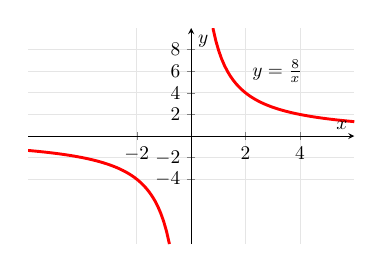
\begin{tikzpicture}[scale=0.7]
	\begin{axis}[
		width=7.5cm, height=5.5cm,
		axis lines=middle,
		xlabel=$x$, ylabel=$y$,
		xmin=-6, xmax=6, ymin=-10, ymax=10,
		xtick={-2,0,2,4}, ytick={-4,-2,2,4,6,8},
		grid=major, grid style={gray!20},
		]
		\node[anchor=west] at (2,6){$y=\frac{8}{x}$};
		\addplot[line width=1.5pt,red,domain=-6:-0.8,samples=50] {8/x};
		\addplot[line width=1.5pt,red,domain=0.8:6,samples=50] {8/x};		
	\end{axis}
\end{tikzpicture}

\vspace{1cm}
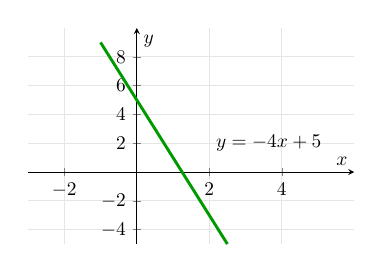
\begin{tikzpicture}[scale=0.7]
	\begin{axis}[
		width=7.5cm, height=5.5cm,
		axis lines=middle,
		xlabel=$x$, ylabel=$y$,
		xmin=-3, xmax=6, ymin=-5, ymax=10,
		xtick={-2,0,2,4}, ytick={-4,-2,2,4,6,8},
		grid=major, grid style={gray!20},
		]


		\addplot[line width=1.5pt,green!60!black,domain=-1:2.5,samples=2] {-4*x+5};
	\node[anchor=west] at (2,2){$y=-4x+5$};
	\end{axis}
\end{tikzpicture}
\hspace{2cm}
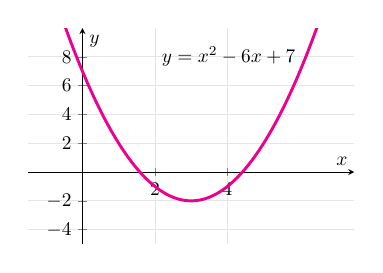
\begin{tikzpicture}[scale=0.7]
	\begin{axis}[
		width=7.5cm, height=5.5cm,
		axis lines=middle,
		xlabel=$x$, ylabel=$y$,
		xmin=-1.5, xmax=7.5, ymin=-5, ymax=10,
		xtick={-2,0,2,4}, ytick={-4,-2,2,4,6,8},
		grid=major, grid style={gray!20},
		]
		
		
		\addplot[line width=1.5pt,magenta,domain=-1:7,samples=100] {(x-3)^2-2};
		\node[anchor=west] at (2,8){$y=x^2-6x+7$};
	\end{axis}
\end{tikzpicture}
\end{center}
\end{frame}

% ========== 第4题 ==========
\begin{frame}[t]{第4题：求函数值}
\textbf{4.} 已知函数 $f(x)=3x^2-5x+2$，求 $f(-\sqrt{2})$，$f(-a)$，$f(a+3)$，$f(a)+f(3)$ 的值。
\end{frame}

\begin{frame}[t]{第4题 解答}
\begin{tcolorbox}[colback=orange!10,colframe=orange,title=\textbf{解:}]
	\begin{align*}
		&f(-\sqrt{2})=3(-\sqrt{2})^2-5(-\sqrt{2})+2=6+5\sqrt{2}+2=8+5\sqrt{2}.\\
		&f(-a)=3(-a)^2-5(-a)+2=3a^2+5a+2.\\
		&f(a+3)=3(a+3)^2-5(a+3)+2=3(a^2+6a+9)-5a-15+2
		=3a^2+13a+14.\\
		&f(a)+f(3)=(3a^2-5a+2)+(27-15+2)=3a^2-5a+16.
	\end{align*}
		

\end{tcolorbox}
\end{frame}

% ========== 第5题 ==========
\begin{frame}[t]{第5题：点与图象的关系}
\textbf{5.} 已知函数 $\displaystyle f(x)=\frac{x+2}{x-6}$。

\vspace{0.8em}
(1) 点 $(3,14)$ 在 $f(x)$ 的图象上吗？

\vspace{0.8em}
(2) 当 $x=4$ 时，求 $f(x)$ 的值。

\vspace{0.8em}
(3) 当 $f(x)=2$ 时，求 $x$ 的值。
\end{frame}

\begin{frame}[t]{第5题 解答}
\begin{tcolorbox}[colback=orange!10,colframe=orange,title=\textbf{解}]
(1) $f(3)=\dfrac{3+2}{3-6}=\dfrac{5}{-3}=-\dfrac{5}{3}\neq 14$，所以点 $(3,14)$ \alert{不在}图象上。

(2) $f(4)=\dfrac{4+2}{4-6}=\dfrac{6}{-2}=-3$。

(3) 令 $\dfrac{x+2}{x-6}=2$，则 $x+2=2(x-6)$，即 $x+2=2x-12$，解得 $x=14$。
\end{tcolorbox}
\end{frame}

% ========== 第6题 ==========
\begin{frame}[t]{第6题：待定系数法}
\textbf{6.} 若 $f(x)=x^2+bx+c$，且 $f(1)=0$，$f(3)=0$，求 $f(-1)$ 的值。
\end{frame}

\begin{frame}[t]{第6题 解答}
\begin{tcolorbox}[colback=orange!10,colframe=orange,title=\textbf{解}]
由 $f(1)=0$，$f(3)=0$ 知 $1$ 和 $3$ 是方程 $x^2+bx+c=0$ 的两根。

由韦达定理：
\[
1+3=-b \quad\Rightarrow\quad b=-4,
\]
\[
1\times 3=c \quad\Rightarrow\quad c=3.
\]
所以 $f(x)=x^2-4x+3=(x-1)(x-3)$。

\vspace{0.5em}
于是
\[
f(-1)=(-1)^2-4(-1)+3=1+4+3=8.
\]
\end{tcolorbox}
\end{frame}

% ========== 第7题 ==========
\begin{frame}[t]{第7题：画分段函数与离散函数图象}
\textbf{7.} 画出下列函数的图象：

\vspace{0.8em}
(1) $\displaystyle f(x)=\begin{cases}0, & x\le 0,\\ 1, & x>0;\end{cases}$

\vspace{1em}
(2) $G(n)=3n+1$，$n\in\{1,2,3\}$。
\end{frame}

\begin{frame}[t]{第7题 解答与图象}
\begin{center}
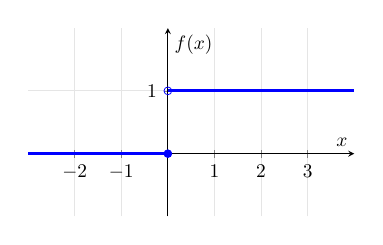
\begin{tikzpicture}[scale=0.7]
\begin{axis}[
    width=7.5cm, height=5cm,
    axis lines=middle,
    xlabel=$x$, ylabel=$f(x)$,
    xmin=-3, xmax=4, ymin=-1, ymax=2,
    xtick={-2,-1,0,1,2,3}, ytick={0,1},
    grid=major, grid style={gray!20},
]
\addplot[line width=1.5pt,blue,domain=-3:0,samples=2] {0};
\addplot[line width=1.5pt,blue,domain=0:4,samples=2] {1};
\addplot[only marks,mark=*,mark size=2pt,blue] coordinates {(0,0)};
\addplot[only marks,mark=o,mark size=2pt,blue] coordinates {(0,1)};
%\node[below right] at (axis cs:3.5,0.8) {(1)};
\end{axis}
\end{tikzpicture}
\hspace{1em}
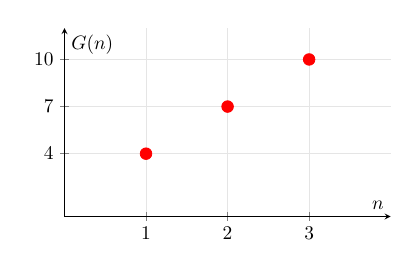
\begin{tikzpicture}[scale=0.7]
\begin{axis}[
    width=7.5cm, height=5cm,
    axis lines=middle,
    xlabel=$n$, ylabel=$G(n)$,
    xmin=0, xmax=4, ymin=0, ymax=12,
    xtick={1,2,3}, ytick={4,7,10},
    grid=major, grid style={gray!20},
]
\addplot[only marks,mark=*,mark size=3pt,red] coordinates {(1,4)(2,7)(3,10)};
%\node[below right] at (axis cs:3.3,1) {(2)};
\end{axis}
\end{tikzpicture}
\end{center}
\end{frame}

% ========== 第8题 ==========
\begin{frame}[t]{第8题：矩形的函数关系}
\textbf{8.} 如图，矩形的面积为 $10$。如果矩形的长为 $x$，宽为 $y$，对角线为 $d$，周长为 $l$，那么你能获得关于这些量的哪些函数？

\vspace{2em}
\begin{center}
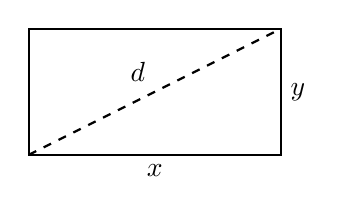
\begin{tikzpicture}[scale=0.8]
\draw[thick] (0,0) rectangle (4,2);
\draw[thick,dashed] (0,0) -- (4,2);
\node[below] at (2,0) {$x$};
\node[right] at (4,1) {$y$};
\node[above left] at (2,1) {$d$};
\end{tikzpicture}
\end{center}
\end{frame}

\begin{frame}[t]{第8题 解答}
\begin{tcolorbox}[colback=orange!10,colframe=orange,title=\textbf{解}]
由矩形面积为 $10$，得：

\vspace{0.5em}
(1) 宽关于长：$\displaystyle y=\frac{10}{x}$，定义域 $(0,+\infty)$；

\vspace{0.5em}
(2) 对角线关于长：$\displaystyle d=\sqrt{x^2+\frac{100}{x^2}}$，定义域$(0,+\infty)$；

\vspace{0.5em}
(3) 周长关于长：$\displaystyle l=2\left(x+\frac{10}{x}\right)$，定义域 $(0,+\infty)$。
\end{tcolorbox}
\end{frame}

% ========== 第9题 ==========
\begin{frame}[t]{第9题：圆柱形容器注液}
\textbf{9.} 一个圆柱形容器的底部直径是 $d$ cm，高是 $h$ cm。现在向容器内每秒注入某种溶液 $v$ cm$^3$。求容器内溶液的高度 $x$（单位：cm）关于注入溶液的时间 $t$（单位：s）的函数解析式，并写出函数的定义域和值域。
\end{frame}

\begin{frame}[t]{第9题 解答}
	\vspace{-2em}
\begin{tcolorbox}[colback=orange!10,colframe=orange,title=\textbf{解}]
容器底面积：$S=\pi\left(\dfrac{d}{2}\right)^2=\dfrac{\pi d^2}{4}$。

\vspace{0.5em}
$t$ 秒注入溶液体积为 $vt$ cm$^3$，故溶液高度：
\[
x=\frac{vt}{S}=\frac{4vt}{\pi d^2}.
\]

\vspace{0.5em}
当溶液注满时 $x=h$，即 $t=\dfrac{\pi d^2 h}{4v}$。

\vspace{0.5em}
\textbf{定义域：} $\left[0,\dfrac{\pi d^2 h}{4v}\right]$；

\vspace{0.3em}
\textbf{值域：} $[0,h]$。
\end{tcolorbox}
\end{frame}

% ========== 第10题 ==========
\begin{frame}[t]{第10题：5分制评分}
\textbf{10.} 一个老师用 $5$ 分制对数学作业评分。一次作业中，第一小组同学按座位序号 $1,2,3,4,5,6$ 的次序，得分依次是 $5,3,4,2,4,5$。你会怎样表示这次作业的得分情况？用 $x,y$ 分别表示序号和对应的得分，$y$ 是 $x$ 的函数吗？如果是，那么它的定义域、值域和对应关系各是什么？
\end{frame}

\begin{frame}[t]{第10题 解答}
\begin{tcolorbox}[colback=orange!10,colframe=orange,title=\textbf{解}]
$y$ 是 $x$ 的函数，可以用列表法表示：

\vspace{0.5em}
\begin{center}
\begin{tabular}{c|cccccc}
$x$ & 1 & 2 & 3 & 4 & 5 & 6 \\
\hline
$y$ & 5 & 3 & 4 & 2 & 4 & 5 \\
\end{tabular}
\end{center}

\vspace{0.5em}
\textbf{定义域：} $\{1,2,3,4,5,6\}$；

\vspace{0.3em}
\textbf{值域：} $\{2,3,4,5\}$；

\vspace{0.3em}
\textbf{对应关系：} 序号 $x$ 对应的得分 $y$ 如上表所示。
\end{tcolorbox}
\end{frame}

% ========== 第11题 ==========
\begin{frame}[t]{第11题：由图象求定义域值域}
\textbf{11.} 函数 $r=f(p)$ 的图象如图所示：

\vspace{0.5em}
(1) 函数 $r=f(p)$ 的定义域、值域各是什么？

\vspace{0.5em}
(2) $r$ 取何值时，只有唯一的 $p$ 值与之对应？

\vspace{1em}
\begin{center}
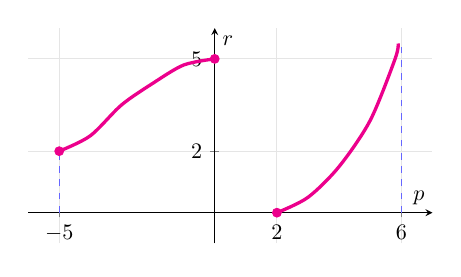
\begin{tikzpicture}[scale=0.8]
\begin{axis}[
    width=8cm, height=5cm,
    axis lines=middle,
    xlabel=$p$, ylabel=$r$,
    xmin=-6, xmax=7, ymin=-1, ymax=6,
    xtick={-5,0,2,6},
    ytick={2,5},
    grid=major, grid style={gray!20},
]
\addplot[line width=1.5pt,magenta,smooth] coordinates {(-5,2)(-4,2.5)(-3,3.5)(-2,4.2)(-1,4.8)(0,5)};
\addplot[line width=1.5pt,magenta,smooth] coordinates {(2,0)(3,0.5)(4,1.5)(5,3)(5.8,5)(5.9,5.5)};
\draw[dashed,blue!60] (axis cs:-5,0) -- (axis cs:-5,2);
\draw[dashed,blue!60] (axis cs:6,0) -- (axis cs:6,5.5);
\addplot[only marks,mark=*,mark size=2pt,magenta] coordinates {(-5,2)(0,5)(2,0)};
\end{axis}
\end{tikzpicture}
\end{center}
\end{frame}

\begin{frame}[t]{第11题 解答}
\begin{tcolorbox}[colback=orange!10,colframe=orange,title=\textbf{解}]
(1) 由图象可知：

\vspace{0.3em}
\textbf{定义域：} $[-5,0]\cup[2,6]$；

\vspace{0.3em}
\textbf{值域：} $[0,5]$。

\vspace{1em}
(2) 当 $r\in[0,2)$ 时，只有唯一的 $p$ 值与之对应（右侧曲线部分）。

\vspace{0.3em}
当 $r\in(2,5]$ 时，有两个 $p$ 值与之对应（左右各一个）。

\vspace{0.3em}
当 $r=2$ 时，有两个 $p$ 值（$p=-5$ 和 $p$ 在右侧某点）。
\end{tcolorbox}
\end{frame}

% ========== 第12题 ==========
\begin{frame}[t]{第12题：画指定定义域值域的函数}
\textbf{12.} 画出定义域为 $\{x\mid -3\le x\le 8,且 x\ne 5\}$，值域为 $\{y\mid -1\le y\le 2, y\ne 0\}$ 的一个函数的图象。

\vspace{0.5em}
(1) 将你的图象和其他同学的相比较，有什么差别吗？

\vspace{0.5em}
(2) 如果平面直角坐标系中点 $P(x,y)$ 的坐标满足 $-3\le x\le 8$，$-1\le y\le 2$，那么其中哪些点不能在图象上？
\end{frame}

\begin{frame}[t]{第12题 参考图象}
\begin{center}
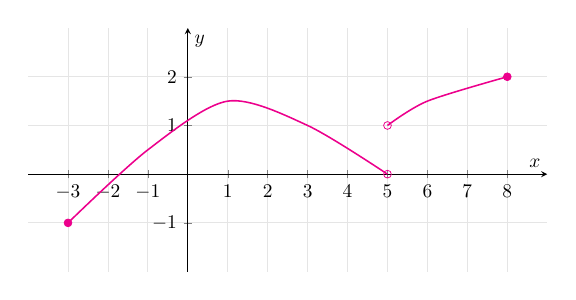
\begin{tikzpicture}[scale=0.7]
\begin{axis}[
    width=11cm, height=6cm,
    axis lines=middle,
    xlabel=$x$, ylabel=$y$,
    xmin=-4, xmax=9, ymin=-2, ymax=3,
    xtick={-3,-2,-1,0,1,2,3,4,5,6,7,8},
    ytick={-1,0,1,2},
    grid=major, grid style={gray!20},
]
% 第一段：[-3, 5)，从(-1, -1)到(2, 2)，到(5, 0)空心
\addplot[thick,magenta,smooth] coordinates {(-3,-1)(-1,0.5)(1,1.5)(3,1)(5,0)};
\addplot[only marks,mark=*,mark size=2pt,magenta] coordinates {(-3,-1)};
\addplot[only marks,mark=o,mark size=2pt,magenta] coordinates {(5,0)};
% 第二段：(5, 8]，从(5, 1)空心到(8, 2)
\addplot[thick,magenta,smooth] coordinates {(5,1)(6,1.5)(8,2)};
\addplot[only marks,mark=o,mark size=2pt,magenta] coordinates {(5,1)};
\addplot[only marks,mark=*,mark size=2pt,magenta] coordinates {(8,2)};
\end{axis}
\end{tikzpicture}
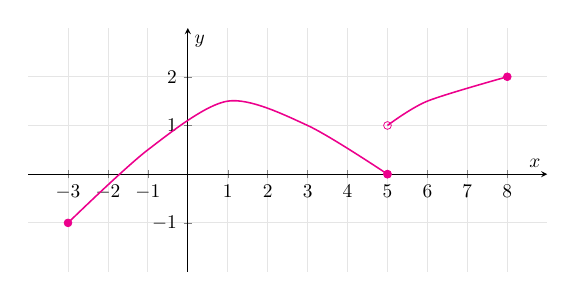
\begin{tikzpicture}[scale=0.7]
	\begin{axis}[
		width=11cm, height=6cm,
		axis lines=middle,
		xlabel=$x$, ylabel=$y$,
		xmin=-4, xmax=9, ymin=-2, ymax=3,
		xtick={-3,-2,-1,0,1,2,3,4,5,6,7,8},
		ytick={-1,0,1,2},
		grid=major, grid style={gray!20},
		]
		% 第一段：[-3, 5)，从(-1, -1)到(2, 2)，到(5, 0)空心
		\addplot[thick,magenta,smooth] coordinates {(-3,-1)(-1,0.5)(1,1.5)(3,1)(5,0)};
		\addplot[only marks,mark=*,mark size=2pt,magenta] coordinates {(-3,-1)(5,0)};
		\addplot[only marks,mark=o,mark size=2pt,magenta] coordinates {(5,0)};
		% 第二段：(5, 8]，从(5, 1)空心到(8, 2)
		\addplot[thick,magenta,smooth] coordinates {(5,1)(6,1.5)(8,2)};
		\addplot[only marks,mark=o,mark size=2pt,magenta] coordinates {(5,1)};
		\addplot[only marks,mark=*,mark size=2pt,magenta] coordinates {(8,2)};
	\end{axis}
\end{tikzpicture}
\end{center}
\end{frame}

\begin{frame}[t]{第12题 解答}
\begin{tcolorbox}[colback=orange!10,colframe=orange,title=\textbf{解}]
(1) 答案不唯一，只要满足定义域和值域要求即可，不同同学画的图象形状可以不同。

\vspace{1em}
(2) 不能在图象上的点是：

\vspace{0.3em}
- 直线 $x=5$ 上的所有点（因为 $x\ne 5$）；

\vspace{0.3em}
- 直线 $y=0$ 上的所有点（因为 $y\ne 0$）。

\vspace{0.5em}
即：$(5,y)$（$-1\le y\le 2$）和 $(x,0)$（$-3\le x\le 8$）这些点都不能在图象上。
\end{tcolorbox}
\end{frame}

% ========== 第13题 ==========
\begin{frame}[t]{第13题：取整函数}
\textbf{13.} 函数 $f(x)=[x]$ 的函数值表示不超过 $x$ 的最大整数，例如，$[-3.5]=-4$，$[2.1]=2$。当 $x\in(-2.5,3]$ 时，写出函数 $f(x)$ 的解析式，并画出函数的图象。
\end{frame}

\begin{frame}[t]{第13题 解答}
\begin{tcolorbox}[colback=orange!10,colframe=orange,title=\textbf{解}]
$f(x)=[x]$ 是取整函数，当 $x\in(-2.5,3]$ 时：

\[
f(x)=
\begin{cases}
-3, & -2.5<x< -2,\\
-2, & -2\le x< -1,\\
-1, & -1\le x< 0,\\
0, & 0 \le x< 1,\\
1, & 1 \le x < 2,\\
2, & 2 \le x < 3.\\
3,	& x=3.
\end{cases}
\]
\end{tcolorbox}
\end{frame}

\begin{frame}[t]{第13题 图象}
\begin{center}
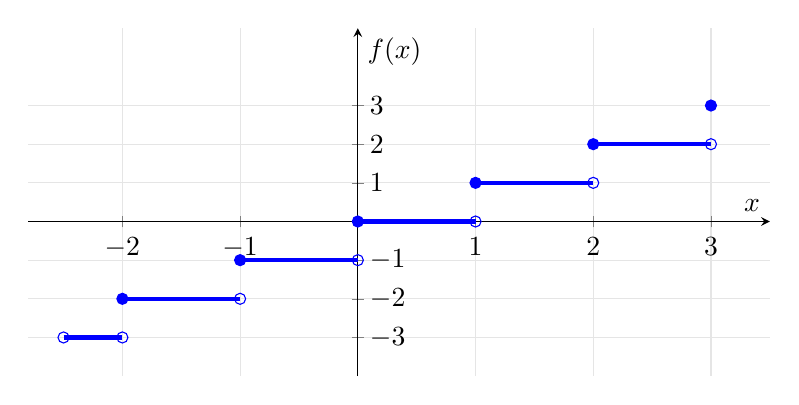
\begin{tikzpicture}[scale=1]
\begin{axis}[
    width=11cm, height=6cm,
    axis lines=middle,
    xlabel=$x$, ylabel=$f(x)$,
    xmin=-2.8, xmax=3.5, ymin=-4, ymax=5,
    xtick={-3,-2,-1,0,1,2,3},
    ytick={-3,-2,-1,0,1,2,3},
    yticklabel style={right,xshift=3pt},
    grid=major, grid style={gray!20},
]
% 阶梯函数：左闭右开
\addplot[line width=1.5pt,blue] coordinates {(-2.5,-3)(-2,-3)};
\addplot[line width=1.5pt,blue] coordinates {(-2,-2)(-1,-2)};
\addplot[line width=1.5pt,blue] coordinates {(-1,-1)(0,-1)};
\addplot[line width=1.5pt,blue] coordinates {(0,0)(1,0)};
\addplot[line width=1.5pt,blue] coordinates {(1,1)(2,1)};
\addplot[line width=1.5pt,blue] coordinates {(2,2)(3,2)};
% 端点：左闭右开
\addplot[only marks,mark=o,mark size=2pt,blue] coordinates {(-2.5,-3)(-2,-3)(-1,-2)(0,-1)(1,0)(2,1)(3,2)};
\addplot[only marks,mark=*,mark size=2pt,blue] coordinates {(-2,-2)(-1,-1)(0,0)(1,1)(2,2)(3,3)};
\end{axis}
\end{tikzpicture}
\end{center}
\end{frame}

% ========== 第14题 ==========
\begin{frame}[t]{第14题：构建问题情境}
\textbf{14.} 构建一个问题情境，使其中的变量关系能用解析式 $\displaystyle y=\frac{1}{2}ax^2\ (a>0)$ 来描述。
\end{frame}

\begin{frame}[t]{第14题 参考示例}
\begin{tcolorbox}[colback=orange!10,colframe=orange,title=\textbf{解}]
示例：一个物体从高处自由下落，下落的距离 $y$（单位：m）与下落时间 $x$（单位：s）的关系为：
\[
y=\frac{1}{2}gx^2,
\]
其中 $g\approx 9.8\,\text{m/s}^2$ 是重力加速度。

\vspace{1em}
其他示例：
- 圆的面积 $S=\pi r^2$（$r$ 为半径）；
- 正方形的面积 $S=a^2$（$a$ 为边长）；
- 匀加速直线运动的位移 $s=\frac{1}{2}at^2$（初速度为0）。
\end{tcolorbox}
\end{frame}

% ========== 第15题 ==========
\begin{frame}[t]{第15题：小岛到城镇的时间}
\textbf{15.} 如图所示，一座小岛距离海岸线上最近的点 $P$ 的距离是 $2$ km，从点 $P$ 沿海岸正东 $12$ km 处有一个城镇。

\vspace{0.5em}
(1) 假设一个人驾驶小船的平均速度为 $3$ km/h，步行速度是 $5$ km/h，$t$（单位：h）表示他从小岛到城镇的时间，$x$（单位：km）表示此人将船停在海岸处距点 $P$ 的距离。请将 $t$ 表示为 $x$ 的函数。

\vspace{0.5em}
(2) 如果将船停在距点 $P$ $4$ km 处，那么从小岛到城镇要多长时间（精确到 $0.1$ h）？
\end{frame}

\begin{frame}[t]{第15题 解答}
	\vspace{-2em}
\begin{tcolorbox}[colback=orange!10,colframe=orange,title=\textbf{解}]
(1) 乘船距离：$\sqrt{x^2+2^2}=\sqrt{x^2+4}$ km，乘船时间：$\dfrac{\sqrt{x^2+4}}{3}$ h；

\vspace{0.3em}
步行距离：$(12-x)$ km，步行时间：$\dfrac{12-x}{5}$ h。

\vspace{0.5em}
总时间：
\[
t=\frac{\sqrt{x^2+4}}{3}+\frac{12-x}{5},\quad x\in[0,12].
\]
(2) 当 $x=4$ 时：
\[
t=\frac{\sqrt{16+4}}{3}+\frac{12-4}{5}=\frac{\sqrt{20}}{3}+\frac{8}{5}\approx\frac{4.47}{3}+1.6\approx 1.5+1.6=3.1\,\text{h}.
\]
约需 \alert{3.1 小时}。
\end{tcolorbox}
\end{frame}

% ========== 第16题 ==========
\begin{frame}[t]{第16题：数集与方程}
\textbf{16.} 给定数集 $A=\mathbf{R}$，$B=(-\infty,0]$，方程 $u^2+2v=0$。

\vspace{0.5em}
(1) 任给 $u\in A$，对应关系 $f$ 使方程①的解 $v$ 与 $u$ 对应，判断 $v=f(u)$ 是否为函数；

\vspace{0.5em}
(2) 任给 $v\in B$，对应关系 $g$ 使方程①的解 $u$ 与 $v$ 对应，判断 $u=g(v)$ 是否为函数。
\end{frame}

\begin{frame}[t]{第16题 解答}
\begin{tcolorbox}[colback=orange!10,colframe=orange,title=\textbf{解}]
(1) 由 $u^2+2v=0$ 得 $\displaystyle v=-\frac{u^2}{2}$。

\vspace{0.3em}
对任意 $u\in\mathbf{R}$，$v$ 有唯一确定的值与之对应，所以 $v=f(u)$ \alert{是}函数。

\vspace{1em}
(2) 由 $u^2+2v=0$ 得 $u=\pm\sqrt{-2v}$。

\vspace{0.3em}
对任意 $v<0$，$u$ 有两个值（正负各一）与之对应，不唯一，所以 $u=g(v)$ \alert{不是}函数。

\vspace{0.3em}
（当 $v=0$ 时，$u=0$ 唯一，但 $v<0$ 时不唯一，整体不是函数。）
\end{tcolorbox}
\end{frame}

% ========== 第17题 ==========
\begin{frame}[t]{第17题：探究函数关系}
\textbf{17.} 探究是否存在函数 $f(x)$，$g(x)$ 满足条件：

\vspace{0.5em}
(1) 定义域相同，值域相同，但对应关系不同；

\vspace{0.5em}
(2) 值域相同，对应关系相同，但定义域不同。
\end{frame}

\begin{frame}[t]{第17题 解答}
\begin{tcolorbox}[colback=orange!10,colframe=orange,title=\textbf{解}]
(1) \textbf{存在。} 例如：
\[
f(x)=x^2,\quad g(x)=x^2+1,
\]
定义域都是 $\mathbf{R}$，但值域不同（$[0,+\infty)$ 和 $[1,+\infty)$）。

\vspace{0.5em}
再例如：$f(x)=x$ 和 $g(x)=|x|$，定义域都是 $\mathbf{R}$，值域都是 $\mathbf{R}$，但对应关系不同。

\vspace{1em}
(2) \textbf{存在。} 例如：
\[
f(x)=x^2,\quad x\in\mathbf{R}; \qquad g(x)=x^2,\quad x\in[0,+\infty).
\]
对应关系相同（都是平方），但值域不同（$[0,+\infty)$ 和 $[0,+\infty)$ 相同）。

\vspace{0.3em}
再例如：$f(x)=x$，$x\in\mathbf{R}$ 和 $g(x)=x$，$x\in[0,1]$，对应关系相同，值域不同。
\end{tcolorbox}
\end{frame}

% ========== 第18题 ==========
\begin{frame}[t]{第18题：圆周率的数字}
\textbf{18.} 在一个展现人脑智力的综艺节目中，一位参加节目的少年能将圆周率 $\pi$ 准确地记忆到小数点后面 $200$ 位，更神奇的是，当主持人说出小数点后面的位数时，这位少年都能准确地说出该数位上的数字。如果记圆周率 $\pi$ 小数点后第 $n$ 位上的数字为 $y$，那么你认为 $y$ 是 $n$ 的函数吗？如果是，请写出函数的定义域、值域与对应关系；如果不是，请说明理由。
\end{frame}

\begin{frame}[t]{第18题 解答}
\begin{tcolorbox}[colback=orange!10,colframe=orange,title=\textbf{解}]
$y$ \alert{是} $n$ 的函数。

\vspace{1em}
\textbf{定义域：} $\{1,2,3,\dots,200\}$（少年能记忆的位数）；

\vspace{0.5em}
\textbf{值域：} $\{0,1,2,3,4,5,6,7,8,9\}$（十个数字）；

\vspace{0.5em}
\textbf{对应关系：} $n$ 对应 $\pi$ 小数点后第 $n$ 位上的数字。

\vspace{1em}
每一个确定的 $n$，都有唯一确定的数字 $y$ 与之对应，符合函数的定义。
\end{tcolorbox}
\end{frame}

\begin{frame}[c]
  \begin{center}
    {\Huge\calligra Thanks!}
  \end{center}
\end{frame}

\end{document}
